Every game has at least two states: playing and game over. \emph{Flat Hunt} has six states in total; three playing states and three game over states (see Figure x). These game states are defined in class \texttt{GAME\_CONSTANTS}:

\begin{lstlisting}
Agent_stuck, Agent_caught, Agent_escapes, Prepare_state, Play_state, 
Move_state: INTEGER is unique
	-- Possible states of the game.
\end{lstlisting}

\begin{figure}[h]
  \centerline{\hbox{
    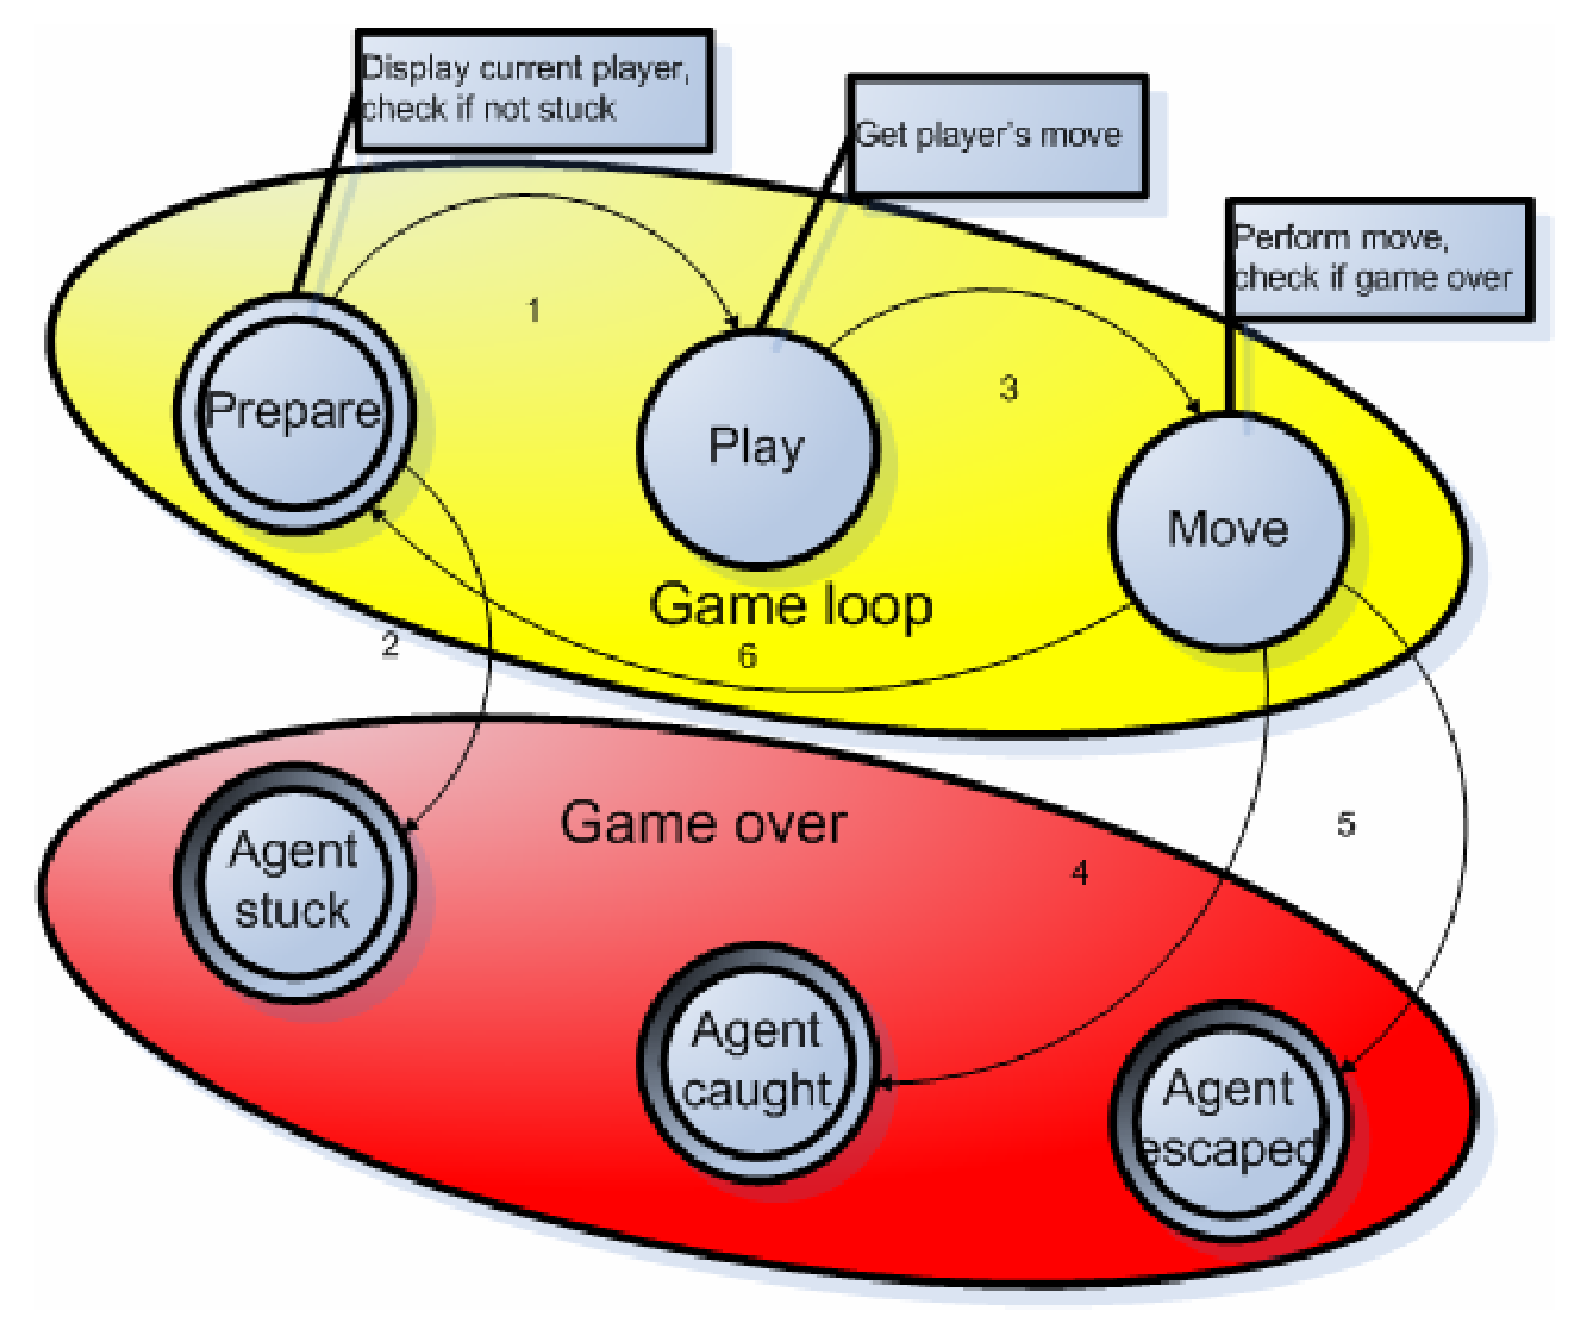
\includegraphics[width=120mm]{gameloop}
  }}
\caption{Game states and loop}
\label{gameloop}
\end{figure}
